\section{Introduction}

Complex Numbers are a very popular and frequently used aspect of Mathematics. Composed of a real part and an imaginary part, they are written in the form \textit{\textbf{x + iy}}. 

\textit{\textbf{x}} denotes the real part and \textit{\textbf{iy}} denotes the imaginary part. Complex numbers can be represented on an \textbf{Argand Diagram}. An \textbf{Argand Diagram} is similar to the \textbf{Cartesian Coordinate System} except that the Real axis and Imaginary axis replace the  \textit{\textbf{X \textit{\textbf{and}} Y}} axis respectively which you would usually expect see on the Cartesian system. This is shown in Figure 1.
\begin{figure}[!htbp]
\begin{center}
\begin{tikzpicture}
    \begin{scope}[thick,font=\scriptsize]
    
    
    \draw [->] (-4,0) -- (4,0) node [above left]  {$\Re\{z\}$};
    \draw [->] (0,-4) -- (0,4) node [below right] {$\Im\{z\}$};

    
    \foreach \n in {-3,...,-1,1,2,...,3}{%
        \draw (\n,-3pt) -- (\n,3pt)   node [above] {$\n$};
        \draw (-3pt,\n) -- (3pt,\n)   node [right] {$\n i$};}
        
    \draw [thick, color=red] (0,0) -- (2,3);
    \draw [color=blue, fill=blue] (2,3) circle(0.05);
    \node [color=black] at (3,3) {$ 2+3i$};
\end{scope}
\end{tikzpicture}
\end{center}
\caption{This Shows the Complex Number \textit{\textbf{2+3i}} plotted on an Argand Diagram}

 
\end{figure}


\section{Properties of Complex Numbers}

All Complex Numbers have a Modulus and an Argument. 

\begin{figure}
These Diagrams Show Illustrations of the Argument and Modulus of a Complex Number:
\begin{minipage}{.5\textwidth}
  \centering
  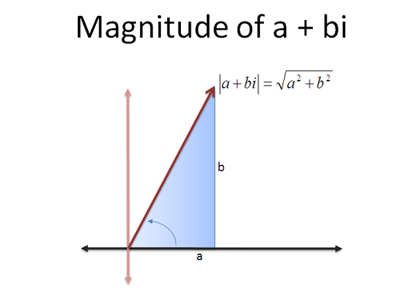
\includegraphics[width=.4\linewidth]{complex_magnitude}
  \captionof{figure}{Modulus of a Complex Number}
  \label{fig:test1}
\end{minipage}%
\begin{minipage}{.5\textwidth}
  \centering
  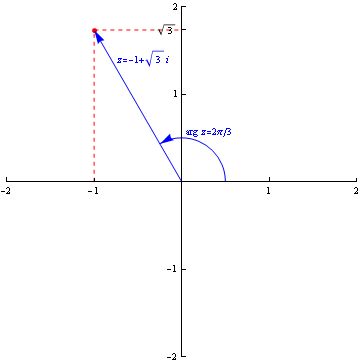
\includegraphics[width=.4\linewidth]{figure_argument}
  \captionof{figure}{Argument of a Complex Number}
  \label{fig:test2}
\end{minipage}
\end{figure}


The Modulus of the Complex Number gives the straight line distance from the origin to the point. The Argument gives the angle between the line representing the complex number and the positive real axis. However the maximum argument is \textit{\textbf{$\pi$}} as when the complex number is below the real axis the argument becomes negative, hence the range of the argument($\theta$) is \textit{\textbf{$\pi$\textless$\theta$$\leqslant$$\pi$}}.

Below is some code which would work out the Modulus and Argument of a complex number in sage.
\begin{verbatim}
z = 32 + 15i
	
    """
    This defines Z as our complex number
    """
abs(z) # this works out the modulus of z. This is done by working out the square root of 32^2 + 15^2.

arg(z) #this works out the argument of z by doing arctan(15/32)

\end{verbatim}

This can be seen working here : http://sage.maths.cf.ac.uk/home/pub/109 

\small

\section{Basic Operations With Complex Numbers}

Addition of complex numbers is self explanatory and is done in the same way as you would add other algebraic terms. The same applies for subtraction. However multiplication is slightly different. When you multiply out the brackets you would obtain an \textit{i}$^2$ term. We know that \textit{i}$^2$ is equivalent to \textbf{-1} so this can be simplified. See below :

\begin{align}
(3+4i)(-4+7i) & =-12+21i-16i+28i^2\nonumber\\
			  & =-12+5i+28i^2\nonumber\\
              & =-12+5i-28\nonumber\\
              & =-40+5i\nonumber\\
\end{align}

Division is also different when involving complex numbers. You must use the complex conjugate of the bottom complex number and times both the numerator and denominator by it. The complex conjugate is the same as the original number except with the opposite sign of the complex part. This makes the bottom multiplication a difference of squares hence the \textit{i} term will eradicated meaning we will be left with only the real and \textit{i}$^2$ term, which as we have seen from the multiplication can be simplified to a pure real term. See below:

\begin{align}
\frac{4+7i}{3-2i}\nonumber & = \frac{4+7i}{3-2i} \cdot \frac{3+2i}{3+2i}\nonumber\\
				  & = \frac{12+21i+8i+14i^2}{9+6i-6i-4i^2}\nonumber\\
                  & = \frac{12+29i-14}{9+4}\nonumber\\
                  & = \frac{-2+29i}{13}\nonumber\\
\end{align}

\section{More Advanced Uses of Complex Numbers}

Complex Numbers are also useful for further things, for example they can be used to plot a locus of points that illustrate something. If we are given these 2 equations:

\begin{equation}
|z| = 4 \nonumber\\
\end{equation}
\begin{equation}
|z-2+i| = |z+2-i|\nonumber\\
\end{equation}
We can use some simple algebra to plot what they describe. This involves replacing the \textit{z} with \textit{x+iy} and then rearranging to form something we can plot.
Once we have done so, this sage code will plot what each of the complex numbers describe:

For the first: 

\begin{verbatim}
f = sqrt(16-x^2) #one solution of the equation found algebraically

g = -sqrt(16-x^2) #second solution of equation found algebraically

plot([f, g], x, -10, 10) #this plots the points and shows a circle centre (0,0) radius 4
\end{verbatim}
For the Second:
\begin{verbatim}
f(x) = 2*x #this sets the function as y = 2x

p = plot(f(x), x, -10, 10) # this tells us what we are going to plot and what range to plot it in

p.show() # this plots what we have told it to plot
\end{verbatim}

This can be seen working in sage here: http://sage.maths.cf.ac.uk/home/pub/111 

\section{Summary}
I have only touched the surface of what Complex numbers can be used for and how useful they are in this short report, but I hope that this has given you an appetite to go on and learn about them even more. They are useful in a wide array of topics, ranging from quantum mechanics to fluid dynamics.
\scriptsize
\section{References}
-Stack Exchange- Help to know how to put images side by side on a page.

-Better Explained Website - Image of Modulus   

-Imperial University Website - Image of Arguments

-Latex Community Forum - Help Drawing the Argand Diagram